\documentclass[11pt,a4paper]{article}

\usepackage[T1]{fontenc}
\usepackage{lmodern}
\usepackage[margin=2.5cm]{geometry}
\usepackage{graphicx}
\usepackage{booktabs}
\usepackage{float}
\usepackage{caption}
\usepackage{subcaption}
\usepackage{makecell}
\usepackage{array}
\usepackage[hidelinks]{hyperref}

% Tables come from docs/build_tables.py (files docs/tables/final_*.tex and the
% dataset tables of phase 1); figures from the notebook outputs.
\graphicspath{{../notebooks/outputs/phase2/}{../notebooks/outputs/inference/}}
\captionsetup{font=small,labelfont=bf}

\newcommand{\reportauthors}{Oscar Fabian Alfonso \quad Kevin Andrey Bueno \\ Oscar Andres Prieto \quad Juan Camilo Martinez}

\title{From Pixels to Predictions\\[0.3em]
\large A comparative framework for Sentinel-2 land-cover classification\\
Final report}
\author{\reportauthors\\[0.3em] ML101 Final Project}
\date{November 27, 2026}

\begin{document}
\maketitle

\begin{abstract}
\noindent
We classify the land cover of a Sentinel-2 scene over Bogot\'a (tile T18NWL,
August 10, 2026) from its ten 20~m bands, using 583,835 pixels labelled by
11,711 reference polygons. Eight models, covering the six architectures of the
brief and two tree ensembles, were tuned with the same ten validations grouped
by polygon and compared on the same test polygons, with the macro F1-score as
the selection criterion so that rare classes count as much as the dominant
one. A Support Vector Machine with a radial kernel on the logarithm of the
bands was selected (validation macro F1 $0.731 \pm 0.042$) and was also the
best model on the test set: overall accuracy 0.936, kappa 0.849 and macro F1
0.685, ahead of the neural network and Gradient Boosting by about 0.012 of
macro F1. Bright and well-represented classes are recognised reliably (F1
between 0.80 and 0.98), while dark area pixels, water and unclassified pixels
remain difficult (F1 0.20 to 0.52). The selected model, trained again on all
the labelled pixels, classified the 30.1 million pixels of the scene into a
georeferenced raster: vegetation covers 73.0\,\% of the 12,056~km$^2$ mapped,
non-vegetated surfaces 15.4\,\% and cloud shadows 8.1\,\%, the latter
overestimated on steep shaded slopes.
\end{abstract}

\section{Introduction}

This project classifies the land cover of a Sentinel-2 scene over Bogot\'a
pixel by pixel, using machine learning models trained on reference polygons.
The work follows the complete chain of a GeoAI application, written in Python
and run outside desktop GIS software:

\begin{enumerate}
  \item build a table of labelled pixels from the satellite bands and the
  reference polygons;
  \item train, tune and compare the six architectures required by the brief
  (Logistic Regression, K-Nearest Neighbors, Naive Bayes, Decision Trees,
  Support Vector Machines and Artificial Neural Networks), together with two
  ensembles of trees, Random Forest and Gradient Boosting;
  \item classify the whole scene with the best model, export the result as a
  georeferenced raster and measure the area of each land-cover class.
\end{enumerate}

The first phase of the project, delivered on November 13, covered the
training dataset and the first three models. This report presents the whole
study.

\section{Study area and data}

\subsection{Sentinel-2 scene}

The scene is a Sentinel-2 Level-2A product (bottom-of-atmosphere
reflectance) over Bogot\'a and the surrounding Andean region, tile T18NWL,
acquired on August 10, 2026. It covers $109.8 \times 109.8$~km. The ten bands
of Table~\ref{tab:bands} were delivered as JPEG~2000 files resampled to 20~m.
Every band is a $5490 \times 5490$ grid of 16-bit unsigned integers in the
coordinate reference system WGS~84 / UTM zone 18N (EPSG:32618); the ten
grids share the same origin, resolution and size, which was checked before
any use.

\begin{table}[H]
\centering\small
\caption{Spectral bands of the scene.}
\label{tab:bands}
\begin{tabular}{lllr}
\toprule
Band & Description & Region & Central wavelength \\
\midrule
B01 & Coastal aerosol & Visible & 443 nm \\
B02 & Blue & Visible & 490 nm \\
B03 & Green & Visible & 560 nm \\
B04 & Red & Visible & 665 nm \\
B05, B06, B07 & Vegetation red edge & Red edge & 705, 740, 783 nm \\
B8A & Narrow near infrared & NIR & 865 nm \\
B11, B12 & Short-wave infrared & SWIR & 1610, 2190 nm \\
\bottomrule
\end{tabular}
\end{table}

The band files store digital numbers. Converting them to reflectance requires
the offset and the scale written in the product metadata, which was not part
of the delivered files, so the models work directly on the digital numbers.
This does not affect the results: the conversion is the same linear change
for every pixel, tree models are not affected by it, and the other models
standardise the bands before training. Only one pixel of the scene has no
data (value 0 in every band).

\subsection{Reference polygons}

The ground truth is a table of 11,711 polygons, each with its geometry, an
identifier and an integer class label. The labels follow the convention of the
brief (Table~\ref{tab:labels}); the polygons cover classes 2 to 10, so classes
0, 1 and 11 cannot be learned and never appear in the predictions.

\begin{table}[H]
\centering\small
\caption{Class labels of the brief. Classes in bold are present in the
reference polygons.}
\label{tab:labels}
\begin{tabular}{cl@{\hspace{2.5em}}cl}
\toprule
Label & Class & Label & Class \\
\midrule
0 & No data & \textbf{6} & \textbf{Water} \\
1 & Saturated or defective & \textbf{7} & \textbf{Unclassified} \\
\textbf{2} & \textbf{Dark area pixels} & \textbf{8} & \textbf{Cloud medium probability} \\
\textbf{3} & \textbf{Cloud shadows} & \textbf{9} & \textbf{Cloud high probability} \\
\textbf{4} & \textbf{Vegetation} & \textbf{10} & \textbf{Thin cirrus} \\
\textbf{5} & \textbf{Not vegetated} & 11 & Snow \\
\bottomrule
\end{tabular}
\end{table}

\section{Training dataset}

\subsection{Construction}

The dataset is built by three Airflow workflows that move the data through
three layers, each one stored and never overwritten by the next:

\begin{enumerate}
  \item \textbf{Source files.} The ten bands are uploaded unchanged to an
  object store (MinIO), and the polygons are loaded into a PostGIS table after
  checking their columns, identifiers, labels and geometries.
  \item \textbf{Extracted pixels.} Every pixel whose centre lies inside a
  polygon is stored with its ten band values, the latitude and longitude of
  its centre, its class and the identifier of its polygon.
  \item \textbf{Training samples.} The extracted pixels are cleaned and
  exported as the TSV file.
\end{enumerate}

The band values are the digital numbers of the band files. The centre of each
pixel is transformed from EPSG:32618 to geographic coordinates (EPSG:4326) to
obtain the latitude and longitude. Three cleaning rules are applied: a pixel
is dropped when any band has no data, a pixel is dropped when polygons of
different classes claim it, and a pixel covered twice by polygons of the same
class is kept once. None of the rules removed anything in this dataset.

\subsection{Resulting table}

The TSV file has 583,835 rows and thirteen columns: \texttt{Latitude},
\texttt{Longitude}, the ten bands and \texttt{Class}
(Table~\ref{tab:sample}). Three checks confirm it: every pixel centre lies
inside its polygon (spatial query in PostGIS); the total area of the polygons
divided by the area of a pixel (400~m$^2$) equals the number of rows; and 900
band values read again from the band files by geographic coordinate match the
table.

\begin{table}[H]
\centering\scriptsize
\setlength{\tabcolsep}{3.5pt}
\caption{First row of the TSV training dataset.}
\label{tab:sample}
\begin{tabular}{rrrrrrrrrrrrr}
\toprule
Latitude & Longitude & B01 & B02 & B03 & B04 & B05 & B06 & B07 & B8A & B11 & B12 & Class \\
\midrule
5.428046467983549 & $-$74.67295509517224 & 1141 & 1805 & 2175 & 2151 & 2747 & 3776 & 4148 & 4498 & 4085 & 3210 & 4 \\
\bottomrule
\end{tabular}
\end{table}

The classes are strongly imbalanced (Table~\ref{tab:classes}). Class 5 (not
vegetated) holds 73.6\,\% of the pixels, class 10 (thin cirrus) has 49 pixels
from a single polygon, and water comes from only 17 polygons.

\begin{table}[H]
\centering\small
\caption{Polygons and pixels per class in the training dataset.}
\label{tab:classes}
\begin{tabular}{clrrr}
\toprule
Class & Land cover & Polygons & Pixels & Share (\%) \\
\midrule
2 & Dark area pixels & 248 & 4,106 & 0.70 \\
3 & Cloud shadows & 58 & 32,712 & 5.60 \\
4 & Vegetation & 1,919 & 46,345 & 7.94 \\
5 & Not vegetated & 8,444 & 429,680 & 73.60 \\
6 & Water & 17 & 8,640 & 1.48 \\
7 & Unclassified & 361 & 6,510 & 1.12 \\
8 & Cloud medium probability & 226 & 25,348 & 4.34 \\
9 & Cloud high probability & 437 & 30,445 & 5.21 \\
10 & Thin cirrus & 1 & 49 & 0.01 \\
\midrule
 & Total & 11,711 & 583,835 & 100.00 \\
\bottomrule
\end{tabular}

\end{table}

\section{Methodology}

\subsection{Test set}

Pixels of the same polygon are neighbours with nearly identical spectra. If
they were split at random, the test set would contain close copies of
training pixels and every score would be overestimated. The data are
therefore split by polygon: every polygon goes entirely to one side. A
stratified group split (one of five folds held out, fixed random seed) keeps
the class proportions as close as whole polygons allow: 468,989 training
pixels and 114,846 test pixels from 2,213 polygons (Table~\ref{tab:split}).

\begin{table}[H]
\centering\small
\caption{Train and test split by polygon.}
\label{tab:split}
\begin{tabular}{crrrr}
\toprule
Class & Train polygons & Train pixels & Test polygons & Test pixels \\
\midrule
2 & 199 & 3,287 & 49 & 819 \\
3 & 44 & 26,169 & 14 & 6,543 \\
4 & 1,540 & 37,075 & 379 & 9,270 \\
5 & 6,892 & 344,571 & 1,552 & 85,109 \\
6 & 11 & 7,764 & 6 & 876 \\
7 & 290 & 5,208 & 71 & 1,302 \\
8 & 171 & 20,511 & 55 & 4,837 \\
9 & 350 & 24,355 & 87 & 6,090 \\
10 & 1 & 49 & 0 & 0 \\
\midrule
Total & 9,498 & 468,989 & 2,213 & 114,846 \\
\bottomrule
\end{tabular}

\end{table}

The test set is used once, at the end, to evaluate the configuration chosen
for each model; it never takes part in a choice. Its scores are therefore an
independent estimate of how each model behaves on polygons it has never
seen. Class 10 comes from a single polygon, which fell in the training set,
so this class cannot be evaluated.

\subsection{Validation folds}

The hyper-parameters of every model are chosen with the training pixels only.
The training polygons are divided into five folds; each candidate
configuration is trained on four of them and scored on the fifth, rotating
until every fold has been scored once. The procedure is repeated with a
second random division, which gives ten validations per candidate. All the
pixels of a polygon stay in the same fold, and the polygons are assigned so
that every fold keeps the class proportions of the training set (no class
share differs by more than 1.9 percentage points). Every model is compared on
exactly the same folds.

\subsection{Models}

A hyper-parameter is a setting fixed before training that controls how a
model learns. For each model, a set of candidate values was defined for the
hyper-parameters that most influence its behaviour, and every combination was
evaluated (Table~\ref{tab:grid}). Models that rely on distances or on
weighted sums of the bands (Logistic Regression, K-Nearest Neighbors, Support
Vector Machines and the neural network) receive the bands standardised to
zero mean and unit variance; the standardisation is learned inside each
training fold, never on the data used to score it.

\paragraph{Feature options.} Two transformations of the bands are evaluated
for the models that benefit from them. The \emph{logarithm} replaces each
value $x$ by $\log(1+x)$, which compresses the very bright values of clouds.
The \emph{spectral indices} add five normalised differences $(a-b)/(a+b)$
widely used in remote sensing: NDVI (B8A, B04) for vegetation, NDWI (B03,
B8A) and MNDWI (B03, B11) for water, NDMI (B8A, B11) for moisture and NBR
(B8A, B12) for dark surfaces. Trees do not need them, because they compare
bands directly.

\paragraph{Class weights.} With \texttt{class\_weight = balanced}, an error on
a rare class costs more during training than an error on a frequent class, in
inverse proportion to the size of the class. It is evaluated for every model
that supports it.

\paragraph{Logistic Regression} is the linear baseline: it separates the
classes with linear boundaries and estimates the probability of each class.
\texttt{C} controls the regularisation: small values give simpler boundaries,
large values follow the training data more closely.

\paragraph{K-Nearest Neighbors} classifies a pixel by the vote of the $k$
training pixels with the most similar spectra. \texttt{n\_neighbors} sets $k$:
few neighbours follow the small classes closely, many neighbours smooth out
noise. \texttt{weights} decides whether every neighbour votes the same or
closer neighbours weigh more. Similarity is measured with the ordinary
(Euclidean) distance between the standardised features. The feature options
change which pixels are close, so they are part of the search.

\paragraph{Naive Bayes} assumes that, within each class, every feature
follows a normal distribution independent of the others, and picks the most
probable class. \texttt{var\_smoothing} adds a small amount to the variances
to keep the computation stable.

\paragraph{Decision Tree} classifies a pixel with a sequence of yes-or-no
questions on the band values. \texttt{max\_depth} limits the number of
successive questions, \texttt{min\_samples\_leaf} sets the minimum number of
training pixels in each final group, which prevents the tree from memorising
individual pixels, and \texttt{criterion} is the measure of class mixture
used to choose each question.

\paragraph{Random Forest} combines 200 trees, each trained on a random
resample of the pixels and looking at a random subset of the bands at each
question (\texttt{max\_features}); the forest predicts the class with the most
votes.

\paragraph{Gradient Boosting} also combines trees, but builds them one after
another, each new tree correcting the errors left by the previous ones, up to
500 trees. \texttt{learning\_rate} sets how strongly each tree corrects,
\texttt{max\_leaf\_nodes} the complexity of each tree and
\texttt{l2\_regularization} a penalty that keeps the corrections moderate.

\paragraph{Support Vector Machine} looks for the boundary that leaves the
widest possible margin between classes. With the radial (\texttt{rbf}) kernel
the boundary can be curved: each training pixel close to the boundary (a
\emph{support vector}) influences the pixels around it, and the reach of that
influence is set from the spread of the features (\texttt{gamma = scale}).
\texttt{C} balances a wide margin against training errors: a large value
follows the training pixels more closely. The feature options are part of the
search.

\paragraph{Artificial Neural Network} is a multilayer perceptron: the
features pass through one or two hidden layers of artificial neurons
(\texttt{hidden\_layer\_sizes}) that learn non-linear combinations of the
bands. It is trained in mini-batches with the Adam optimiser and stops when
the score on 10\,\% of its training pixels, set aside for this purpose, stops
improving. \texttt{alpha} is a penalty on large weights that limits
overfitting. The network always receives the logarithm of the bands and the
spectral indices, the feature options that worked best for the other
continuous models.

\begin{table}[H]
\centering\footnotesize
\caption{Candidate values of the hyper-parameters of each model. Every
combination was evaluated.}
\label{tab:grid}
\begin{tabular}{llr}
\toprule
Model & Candidate values & Combinations \\
\midrule
Logistic Regression & \makecell[l]{\texttt{indices}: False, True \\ \texttt{C}: 0.01, 0.1, 1, 10 \\ \texttt{class\_weight}: None, balanced} & 16 \\ \addlinespace
K-Nearest Neighbors & \makecell[l]{\texttt{indices}: False, True \\ \texttt{log}: False, True \\ \texttt{n\_neighbors}: 5, 15, 25, 41 \\ \texttt{weights}: uniform, distance} & 32 \\ \addlinespace
Naive Bayes & \makecell[l]{\texttt{indices}: False, True \\ \texttt{log}: False, True \\ \texttt{var\_smoothing}: 10 values, 1e-12 to 0.001 (log scale)} & 40 \\ \addlinespace
Decision Tree & \makecell[l]{\texttt{class\_weight}: None, balanced \\ \texttt{criterion}: gini, entropy \\ \texttt{max\_depth}: 10, 15, 20, None \\ \texttt{min\_samples\_leaf}: 1, 5, 20, 50} & 64 \\ \addlinespace
Random Forest & \makecell[l]{\texttt{class\_weight}: None, balanced\_subsample \\ \texttt{max\_depth}: 20, None \\ \texttt{max\_features}: sqrt, 0.5 \\ \texttt{min\_samples\_leaf}: 1, 5} & 16 \\ \addlinespace
Gradient Boosting & \makecell[l]{\texttt{class\_weight}: None, balanced \\ \texttt{l2\_regularization}: 0, 1 \\ \texttt{learning\_rate}: 0.05, 0.1, 0.2 \\ \texttt{max\_leaf\_nodes}: 31, 63, 127} & 36 \\ \addlinespace
Support Vector Machine & \makecell[l]{\texttt{indices}: False, True \\ \texttt{log}: False, True \\ \texttt{C}: 10, 100, 1000} & 12 \\ \addlinespace
Neural Network (MLP) & \makecell[l]{\texttt{class\_weight}: None, balanced \\ \texttt{alpha}: 1e-04, 0.001 \\ \texttt{hidden\_layer\_sizes}: (64,), (128, 64)} & 8 \\
\bottomrule
\end{tabular}

\end{table}

Random Forest, Gradient Boosting, K-Nearest Neighbors, the Support Vector
Machine and the neural network are much more costly to train or to apply than
the other models. Their candidate combinations were compared on a quarter of
the training pixels, drawn with the same class proportions and kept in the
same folds, and the selected configuration was then trained on all the
training pixels. Every model, including these five, is therefore chosen on the
same ten validations and evaluated on the same test set.

\subsection{Evaluation metrics and selection criterion}

A classifier that always predicts class 5 reaches an overall accuracy of 0.74
without learning anything, so accuracy alone cannot tell a good model from a
poor one. The following metrics are reported:

\begin{itemize}
  \item \textbf{Overall accuracy (OA)}: the share of pixels classified
  correctly.
  \item \textbf{Cohen's kappa}: the agreement between prediction and reference
  beyond what chance alone would give; 0 for the classifier that always
  predicts the most frequent class.
  \item \textbf{Precision} of a class: of the pixels predicted as that class,
  the share that truly belongs to it (reliability).
  \item \textbf{Recall} of a class: of the pixels of that class, the share the
  model recovers (completeness).
  \item \textbf{F1-score}: the harmonic mean of precision and recall.
  \item \textbf{Macro average}: the simple mean over classes 2 to 9, so every
  class counts the same; the \textbf{weighted average} weights each class by
  its number of pixels.
  \item \textbf{Confusion matrix}: reference classes in rows, predicted classes
  in columns.
\end{itemize}

The hyper-parameters of each model, and the model used to map the scene, are
chosen by the \textbf{macro F1 averaged over the ten validations}, so the rare
classes weigh as much as the dominant one. The classifier that always predicts
class 5 is included as a baseline.

\section{Results}

\subsection{Selected hyper-parameters}

Table~\ref{tab:selected} lists the configuration that obtained the best
average macro F1 over the ten validations for each model. Three patterns
repeat across models. The logarithm of the bands was selected by every model
for which it was evaluated, because it brings the very bright cloud pixels
closer to the rest. Class weights were selected only for Logistic Regression
and Random Forest; the other models scored higher without them. Trees need a minimum number of pixels per final group (20 for the
single tree, 5 in the forest), which stops them from memorising individual
pixels.

\begin{table}[H]
\centering\small
\caption{Selected configuration of each model.}
\label{tab:selected}
\begin{tabular}{>{\raggedright\arraybackslash}l>{\raggedright\arraybackslash}p{10.5cm}}
\toprule
Model & Selected configuration \\
\midrule
Logistic Regression & \texttt{indices} = True, \texttt{C} = 1, \texttt{class\_weight} = balanced \\
K-Nearest Neighbors & \texttt{indices} = False, \texttt{log} = True, \texttt{n\_neighbors} = 5, \texttt{weights} = distance \\
Naive Bayes & \texttt{indices} = True, \texttt{log} = True, \texttt{var\_smoothing} = 1e-06 \\
Decision Tree & \texttt{class\_weight} = None, \texttt{criterion} = gini, \texttt{max\_depth} = None, \texttt{min\_samples\_leaf} = 20 \\
Random Forest & \texttt{class\_weight} = balanced\_subsample, \texttt{max\_depth} = None, \texttt{max\_features} = 0.5, \texttt{min\_samples\_leaf} = 5 \\
Gradient Boosting & \texttt{class\_weight} = None, \texttt{l2\_regularization} = 1, \texttt{learning\_rate} = 0.1, \texttt{max\_leaf\_nodes} = 31 \\
Support Vector Machine & \texttt{indices} = False, \texttt{log} = True, \texttt{C} = 1000 \\
Neural Network (MLP) & \texttt{class\_weight} = None, \texttt{alpha} = 1e-04, \texttt{hidden\_layer\_sizes} = (128, 64) \\
\bottomrule
\end{tabular}

\end{table}

\subsection{Validation}

Table~\ref{tab:cv} and Figure~\ref{fig:cv} summarise the ten validations of
the selected configurations. The Support Vector Machine has the highest
average macro F1 (0.731), followed by the neural network (0.710), Gradient
Boosting (0.705) and Random Forest (0.703). The spread across validations
($\pm 0.03$ to $0.05$) is as large as the differences between these four
models, because it comes mostly from the polygons that fall in each fold: the
same two validations are the hardest for every model. Compared validation by
validation, however, the Support Vector Machine has the highest macro F1 in
all ten (tied with the neural network in one), so its advantage is consistent
and not the result of a single favourable fold.

\begin{table}[H]
\centering\small
\caption{Validation scores of the selected configurations: mean over the ten
validations (macro F1 with its standard deviation). The selected model is in
bold.}
\label{tab:cv}
\begin{tabular}{lrrr}
\toprule
Model & Macro F1 & OA & Kappa \\
\midrule
Logistic Regression & 0.6239 $\pm$ 0.0303 & 0.8510 & 0.7052 \\
K-Nearest Neighbors & 0.6935 $\pm$ 0.0304 & 0.9160 & 0.8082 \\
Naive Bayes & 0.6040 $\pm$ 0.0251 & 0.8506 & 0.6928 \\
Decision Tree & 0.6754 $\pm$ 0.0373 & 0.9134 & 0.8032 \\
Random Forest & 0.7033 $\pm$ 0.0357 & 0.9133 & 0.8128 \\
Gradient Boosting & 0.7049 $\pm$ 0.0396 & 0.9234 & 0.8250 \\
\textbf{Support Vector Machine} & \textbf{0.7307 $\pm$ 0.0416} & \textbf{0.9294} & \textbf{0.8385} \\
Neural Network (MLP) & 0.7098 $\pm$ 0.0494 & 0.9275 & 0.8347 \\
\bottomrule
\end{tabular}

\end{table}

\begin{figure}[H]
\centering
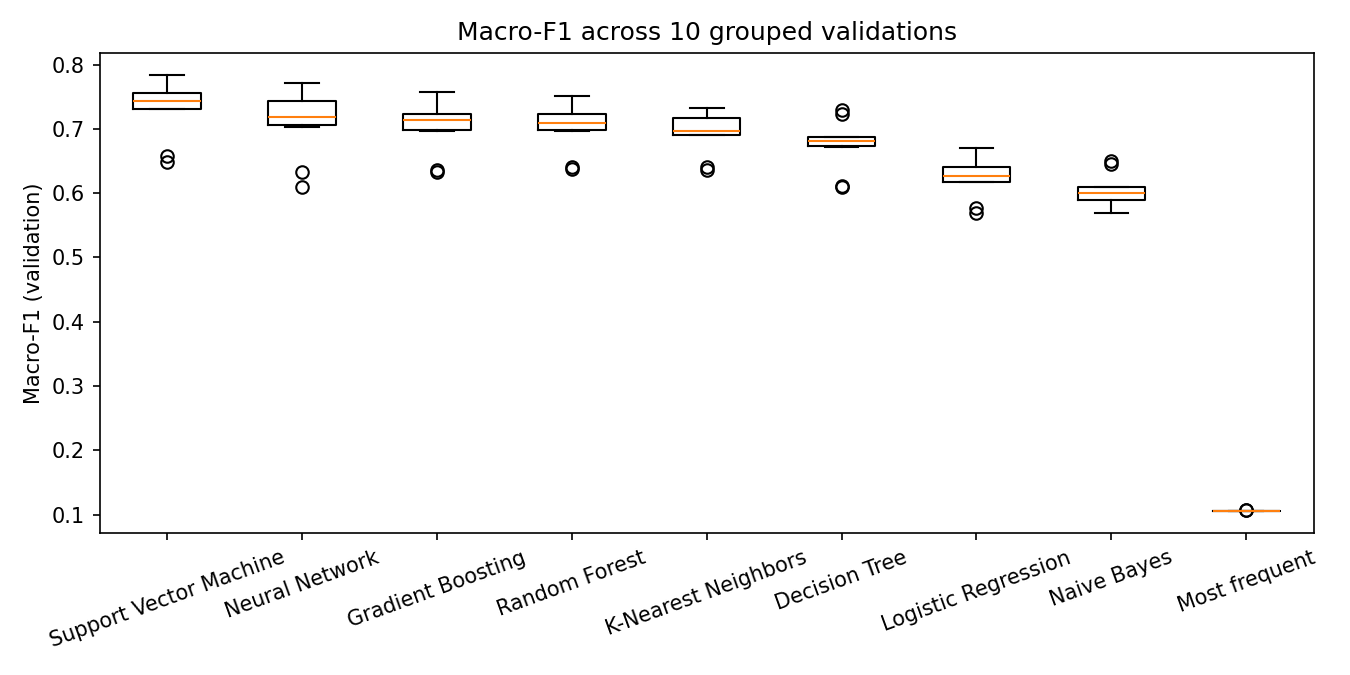
\includegraphics[width=0.9\linewidth]{cv_f1_macro_boxplot}
\caption{Macro F1 of the selected configuration of each model in the ten
validations. The baseline always predicts class 5.}
\label{fig:cv}
\end{figure}

\subsection{Test set}

Table~\ref{tab:holdout} is the summary required by the brief: every model,
trained on all the training pixels with its selected configuration, evaluated
once on the 114,846 test pixels. The Support Vector Machine is the best model
on every metric except macro recall, so the test set confirms the choice made
on the validations. Its overall accuracy (0.936) and kappa (0.849) mean that
it agrees with the reference far beyond chance, and its weighted F1 (0.933)
shows that the frequent classes are classified very well. The neural network
and Gradient Boosting follow within 0.013 of macro F1; Random Forest, the
single tree and K-Nearest Neighbors form a second group; Naive Bayes and
Logistic Regression, the two models with the simplest boundaries, are clearly
below. Every model is far above the baseline, whose kappa is 0.

\begin{table}[H]
\centering\small
\caption{Test-set results of every model, ordered by macro F1. Macro averages
are over classes 2 to 9; the selected model is in bold.}
\label{tab:holdout}
\begin{tabular}{lrrrrrr}
\toprule
Model & OA & Kappa & \makecell{Macro\\precision} & \makecell{Macro\\recall} & \makecell{Macro\\F1} & \makecell{Weighted\\F1} \\
\midrule
\textbf{Support Vector Machine} & \textbf{0.9356} & \textbf{0.8492} & \textbf{0.7170} & \textbf{0.6608} & \textbf{0.6848} & \textbf{0.9330} \\
Neural Network (MLP) & 0.9329 & 0.8435 & 0.6960 & 0.6536 & 0.6725 & 0.9309 \\
Gradient Boosting & 0.9332 & 0.8445 & 0.6973 & 0.6543 & 0.6722 & 0.9308 \\
Random Forest & 0.9212 & 0.8253 & 0.6470 & 0.6990 & 0.6685 & 0.9246 \\
Decision Tree & 0.9182 & 0.8100 & 0.6624 & 0.6314 & 0.6443 & 0.9159 \\
K-Nearest Neighbors & 0.9221 & 0.8182 & 0.6650 & 0.6274 & 0.6426 & 0.9196 \\
Naive Bayes & 0.8442 & 0.6798 & 0.5712 & 0.6441 & 0.5914 & 0.8681 \\
Logistic Regression & 0.8457 & 0.6925 & 0.5608 & 0.6794 & 0.5787 & 0.8748 \\
\midrule
Always class 5 (baseline) & 0.7411 & 0.0000 & 0.0926 & 0.1250 & 0.1064 & 0.6309 \\
\bottomrule
\end{tabular}

\end{table}

The test scores are slightly lower than the validation averages (macro F1
0.685 against 0.731 for the selected model) because the test set holds few
polygons of the rare classes (six of water, fourteen of cloud shadows), and a
single difficult polygon weighs heavily on their F1. The gap between training and test
accuracy of the selected model is small (0.952 against 0.936), so it does not
overfit the training pixels.

\subsection{Results per class}

Table~\ref{tab:f1class} shows the F1-score of every class. The Support Vector
Machine is the best model for five of the eight classes; the neural network is
marginally better for vegetation, Gradient Boosting for high-probability
clouds and Naive Bayes for water. Not-vegetated surfaces and high-probability clouds are recognised
almost perfectly (F1 0.96 to 0.98); cloud shadows, vegetation and
medium-probability clouds are recognised well (0.80 to 0.85). Three classes
remain difficult for every model: unclassified pixels (best F1 0.52), dark
area pixels (0.33) and water (0.49 at best, 0.20 for the selected model).

\begin{table}[H]
\centering\small
\caption{F1-score per class on the test set. The best value of each class is
in bold.}
\label{tab:f1class}
\begin{tabular}{clrrrrrrrr}
\toprule
Class & Land cover & LR & KNN & NB & DT & RF & GB & SVM & ANN \\
\midrule
2 & Dark area pixels & 0.116 & 0.234 & 0.057 & 0.209 & 0.300 & 0.290 & \textbf{0.333} & 0.311 \\
3 & Cloud shadows & 0.754 & 0.810 & 0.777 & 0.790 & 0.824 & 0.841 & \textbf{0.851} & 0.841 \\
4 & Vegetation & 0.769 & 0.808 & 0.740 & 0.796 & 0.839 & 0.840 & 0.839 & \textbf{0.846} \\
5 & Not vegetated & 0.928 & 0.970 & 0.929 & 0.968 & 0.969 & 0.974 & \textbf{0.975} & 0.974 \\
6 & Water & 0.175 & 0.186 & \textbf{0.494} & 0.214 & 0.232 & 0.204 & 0.197 & 0.180 \\
7 & Unclassified & 0.324 & 0.455 & 0.371 & 0.517 & 0.472 & 0.487 & \textbf{0.521} & 0.484 \\
8 & Cloud medium probability & 0.622 & 0.724 & 0.458 & 0.714 & 0.749 & 0.778 & \textbf{0.804} & 0.795 \\
9 & Cloud high probability & 0.942 & 0.953 & 0.906 & 0.946 & 0.963 & \textbf{0.964} & 0.959 & 0.949 \\
\bottomrule
\end{tabular}

\end{table}

Precision and recall separate the two sides of the F1-score
(Tables~\ref{tab:precision} and~\ref{tab:recall}). The Support Vector Machine
has the highest precision for five classes: when it assigns a pixel to dark
area, vegetation, unclassified or cloud, it is right more often than any other
model. Recall is where the models trained with class weights stand out:
Logistic Regression recovers the most dark area pixels (0.44) and unclassified
pixels (0.75), and Random Forest the most vegetation and cloud pixels. They
pay for it in precision, since every extra rare-class pixel they find comes
with many false alarms (Logistic Regression has a precision of 0.07 for dark
area pixels). The selected model sits on the other side of this trade-off: it
is reliable when it predicts a rare class, but it misses a large part of them.
Water is the extreme case: every model except Naive Bayes recovers at most a
quarter of its pixels, and none is right in more than half of its water
predictions.

\begin{table}[H]
\centering\small
\caption{Precision per class on the test set (of the pixels predicted as a
class, the share that belongs to it). The best value of each class is in
bold.}
\label{tab:precision}
\begin{tabular}{clrrrrrrrr}
\toprule
Class & Land cover & LR & KNN & NB & DT & RF & GB & SVM & ANN \\
\midrule
2 & Dark area pixels & 0.067 & 0.323 & 0.034 & 0.283 & 0.286 & 0.386 & \textbf{0.433} & 0.365 \\
3 & Cloud shadows & 0.880 & 0.852 & 0.850 & 0.803 & 0.859 & 0.875 & 0.873 & \textbf{0.888} \\
4 & Vegetation & 0.703 & 0.793 & 0.690 & 0.781 & 0.790 & 0.821 & \textbf{0.834} & 0.822 \\
5 & Not vegetated & \textbf{0.993} & 0.963 & 0.977 & 0.963 & 0.983 & 0.968 & 0.966 & 0.967 \\
6 & Water & 0.162 & 0.194 & \textbf{0.448} & 0.243 & 0.213 & 0.237 & 0.230 & 0.198 \\
7 & Unclassified & 0.207 & 0.465 & 0.273 & 0.529 & 0.384 & 0.517 & \textbf{0.586} & 0.538 \\
8 & Cloud medium probability & 0.550 & 0.797 & 0.397 & 0.754 & 0.714 & 0.821 & \textbf{0.853} & 0.833 \\
9 & Cloud high probability & 0.923 & 0.932 & 0.900 & 0.944 & 0.947 & 0.952 & \textbf{0.961} & 0.957 \\
\bottomrule
\end{tabular}

\end{table}

\begin{table}[H]
\centering\small
\caption{Recall per class on the test set (of the pixels of a class, the share
the model recovers). The best value of each class is in bold.}
\label{tab:recall}
\begin{tabular}{clrrrrrrrr}
\toprule
Class & Land cover & LR & KNN & NB & DT & RF & GB & SVM & ANN \\
\midrule
2 & Dark area pixels & \textbf{0.441} & 0.183 & 0.173 & 0.166 & 0.316 & 0.232 & 0.270 & 0.271 \\
3 & Cloud shadows & 0.659 & 0.773 & 0.715 & 0.778 & 0.791 & 0.809 & \textbf{0.830} & 0.798 \\
4 & Vegetation & 0.848 & 0.823 & 0.798 & 0.811 & \textbf{0.893} & 0.861 & 0.845 & 0.872 \\
5 & Not vegetated & 0.871 & 0.977 & 0.885 & 0.973 & 0.955 & 0.980 & \textbf{0.983} & 0.981 \\
6 & Water & 0.189 & 0.179 & \textbf{0.549} & 0.191 & 0.255 & 0.179 & 0.172 & 0.166 \\
7 & Unclassified & \textbf{0.751} & 0.445 & 0.580 & 0.505 & 0.614 & 0.459 & 0.469 & 0.440 \\
8 & Cloud medium probability & 0.714 & 0.664 & 0.541 & 0.679 & \textbf{0.788} & 0.738 & 0.760 & 0.760 \\
9 & Cloud high probability & 0.961 & 0.974 & 0.912 & 0.948 & \textbf{0.980} & 0.975 & 0.957 & 0.941 \\
\bottomrule
\end{tabular}

\end{table}

The confusion matrix of the selected model (Table~\ref{tab:confusion}, and
Figure~\ref{fig:allconfusion} for every model, normalised by reference class)
explains these difficulties. Three quarters of the
water pixels are predicted as not vegetated, and one fifth of the unclassified
pixels as water: in this scene water bodies are small, often turbid or mixed
with their banks, and at 20~m their spectra look like those of dark built-up
or bare surfaces. Dark area pixels are spread over every neighbouring class,
because a dark pixel can be a shadow, wet soil, dense vegetation or water.
Naive Bayes, which uses the water indices among its features, is the only
model that recovers more than half of the water pixels, but at the cost of
many false detections in other classes (its precision for dark area pixels is
0.03).

\begin{table}[H]
\centering\small
\caption{Confusion matrix of the Support Vector Machine on the test set
(pixels; reference classes in rows, predicted classes in columns). Class 10
has no test pixels.}
\label{tab:confusion}
\begin{tabular}{crrrrrrrrrr}
\toprule
Ref. & 2 & 3 & 4 & 5 & 6 & 7 & 8 & 9 & 10 & Total \\
\midrule
2 & 221 & 99 & 135 & 227 & 19 & 114 & 4 & 0 & 0 & 819 \\
3 & 92 & 5,431 & 565 & 305 & 1 & 80 & 69 & 0 & 0 & 6,543 \\
4 & 72 & 231 & 7,830 & 1,025 & 0 & 19 & 93 & 0 & 0 & 9,270 \\
5 & 43 & 88 & 636 & 83,704 & 228 & 115 & 284 & 9 & 2 & 85,109 \\
6 & 1 & 9 & 0 & 648 & 151 & 66 & 1 & 0 & 0 & 876 \\
7 & 74 & 109 & 2 & 185 & 258 & 610 & 64 & 0 & 0 & 1,302 \\
8 & 7 & 253 & 222 & 410 & 0 & 37 & 3,677 & 230 & 1 & 4,837 \\
9 & 0 & 0 & 0 & 141 & 0 & 0 & 118 & 5,831 & 0 & 6,090 \\
10 & 0 & 0 & 0 & 0 & 0 & 0 & 0 & 0 & 0 & 0 \\
\midrule
Total & 510 & 6,220 & 9,390 & 86,645 & 657 & 1,041 & 4,310 & 6,070 & 3 & 114,846 \\
\bottomrule
\end{tabular}

\end{table}

\begin{figure}[H]
\centering
\begin{subfigure}{0.24\linewidth}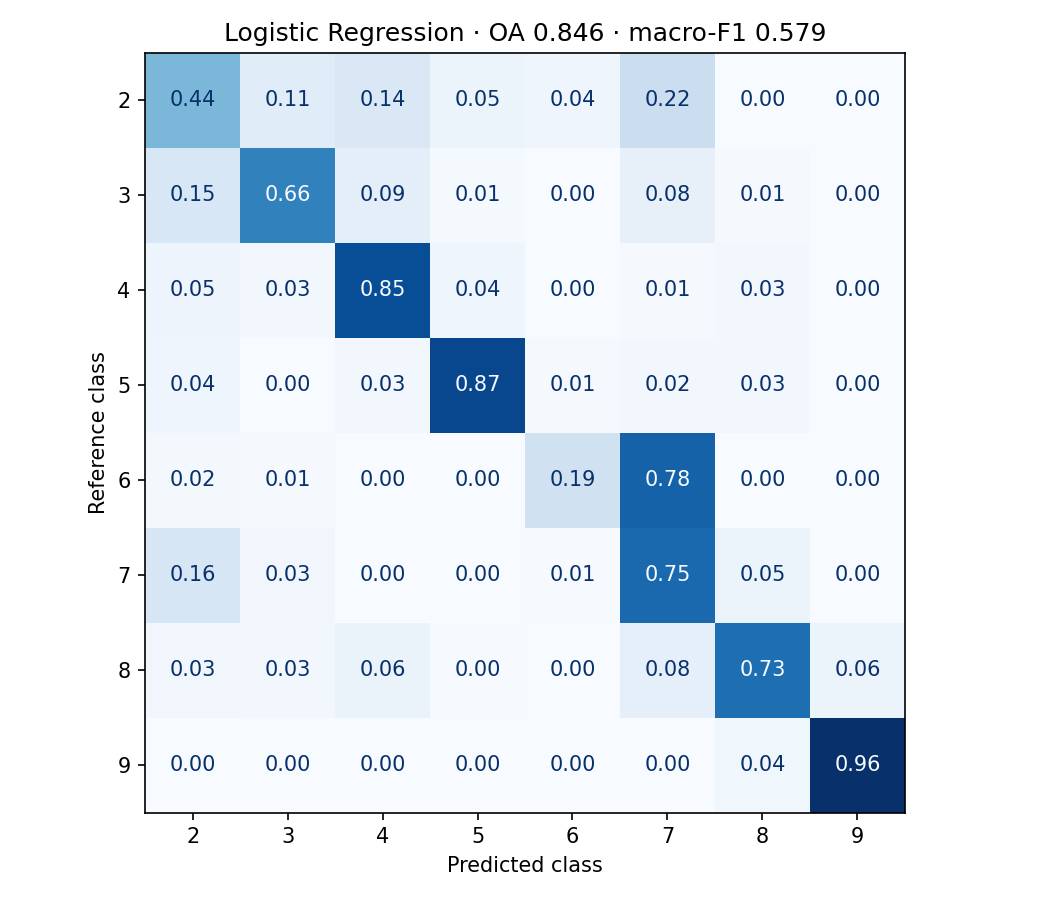
\includegraphics[width=\linewidth]{confusion_matrix_logistic_regression}\end{subfigure}\hfill
\begin{subfigure}{0.24\linewidth}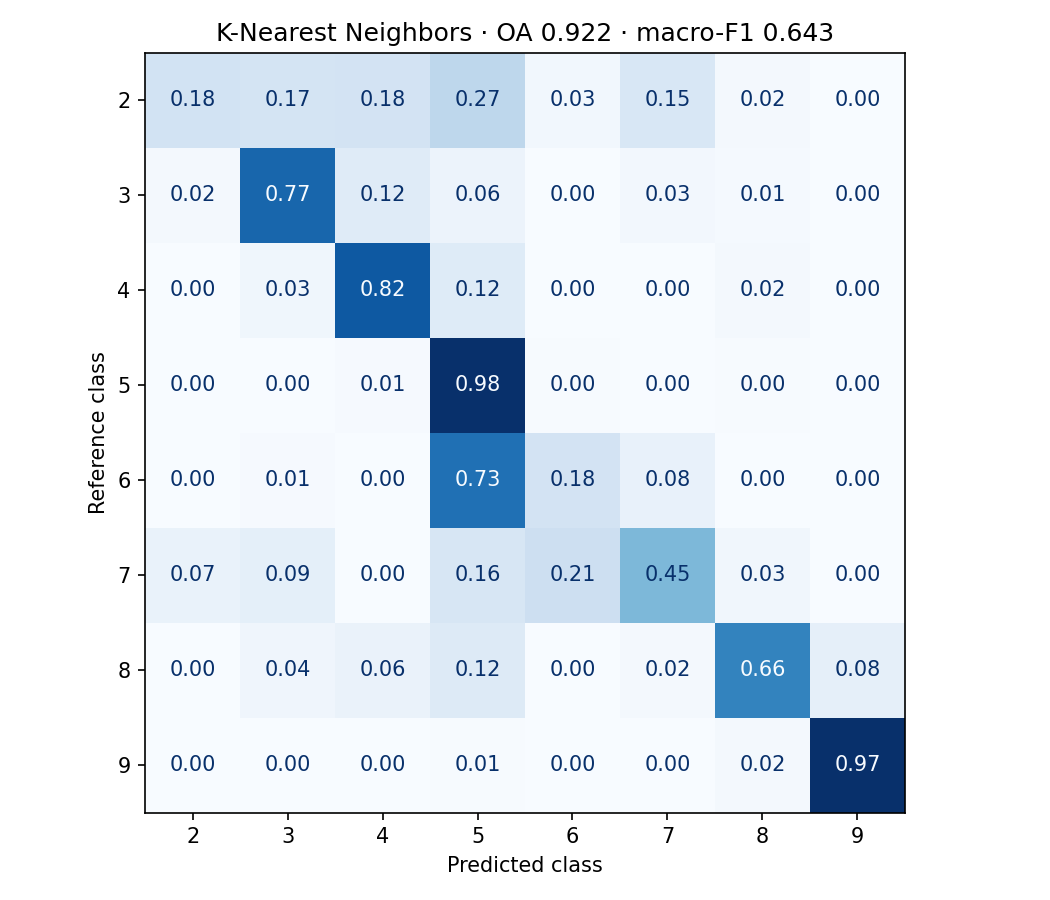
\includegraphics[width=\linewidth]{confusion_matrix_knn}\end{subfigure}\hfill
\begin{subfigure}{0.24\linewidth}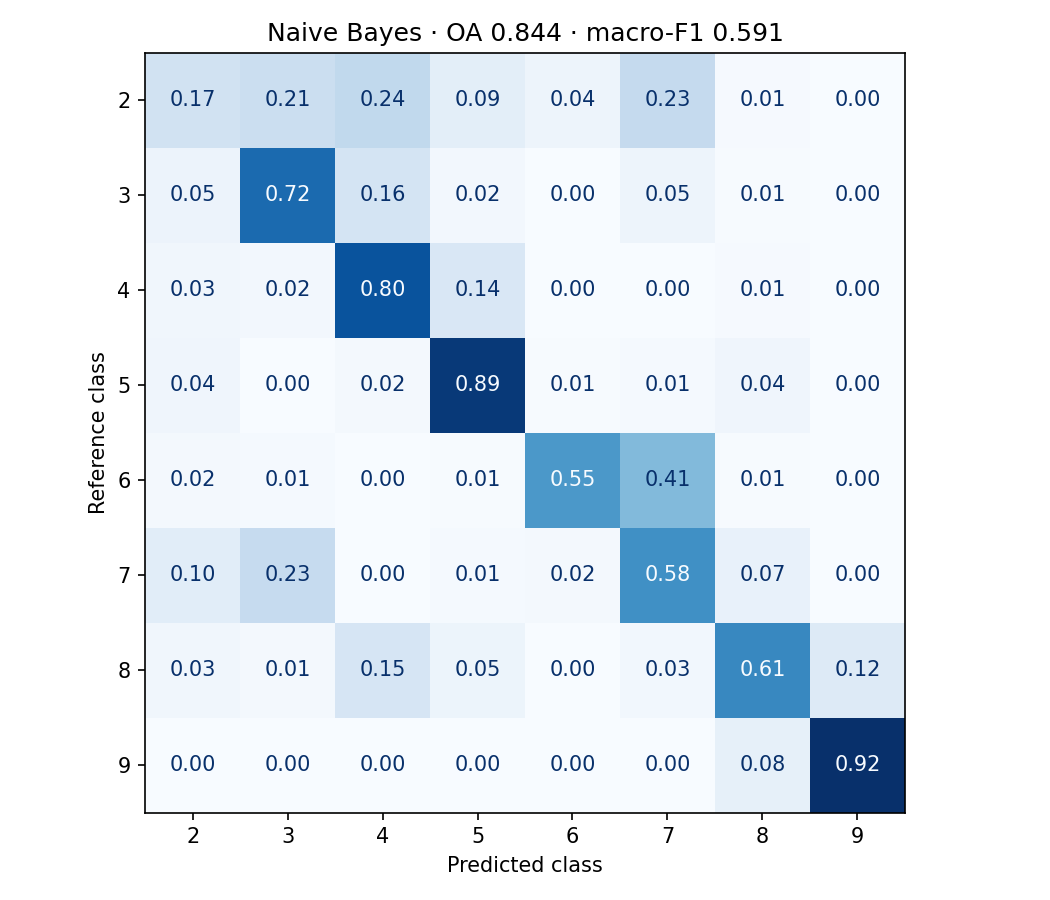
\includegraphics[width=\linewidth]{confusion_matrix_naive_bayes}\end{subfigure}\hfill
\begin{subfigure}{0.24\linewidth}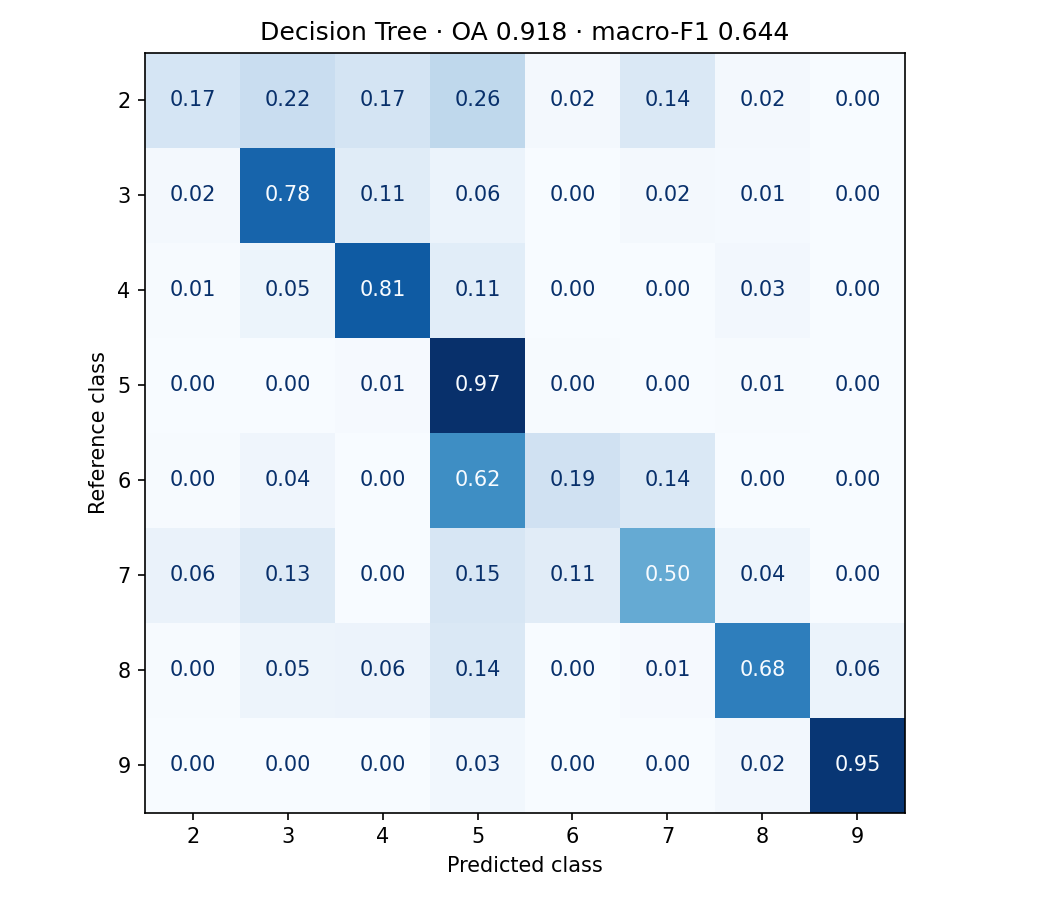
\includegraphics[width=\linewidth]{confusion_matrix_decision_tree}\end{subfigure}\\[0.4em]
\begin{subfigure}{0.24\linewidth}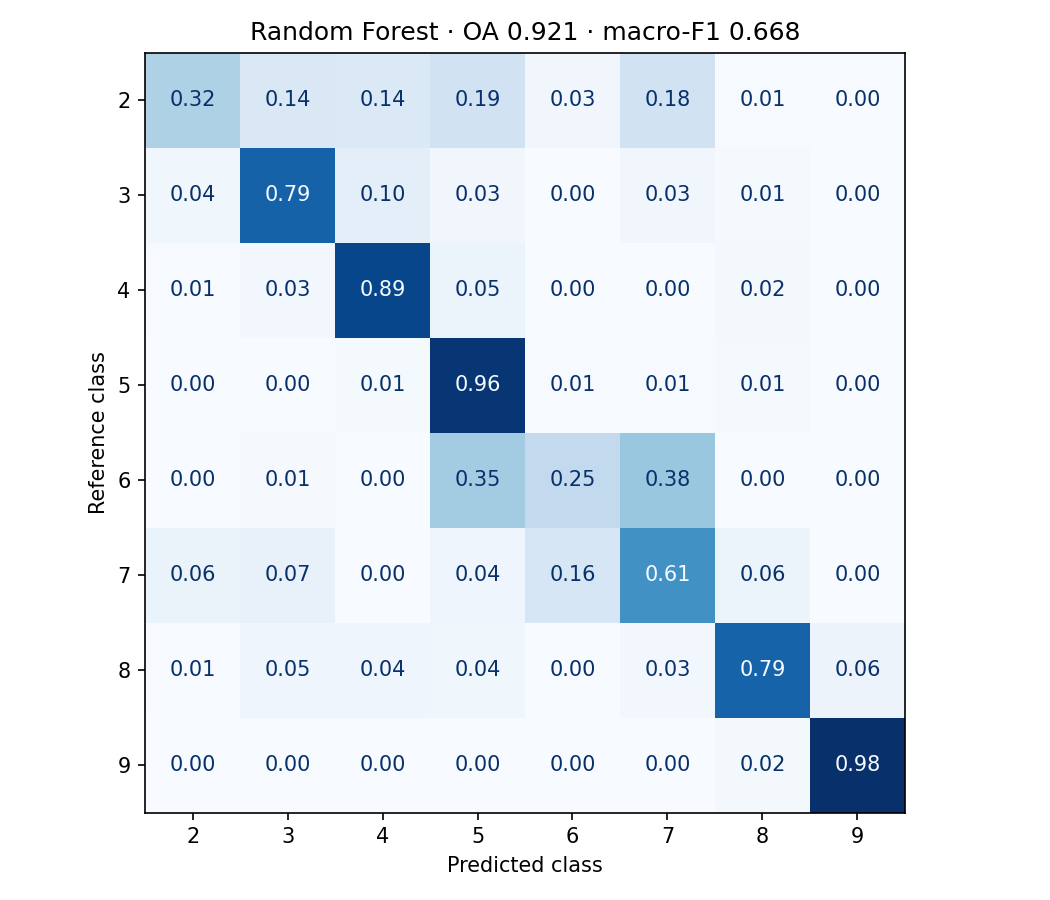
\includegraphics[width=\linewidth]{confusion_matrix_random_forest}\end{subfigure}\hfill
\begin{subfigure}{0.24\linewidth}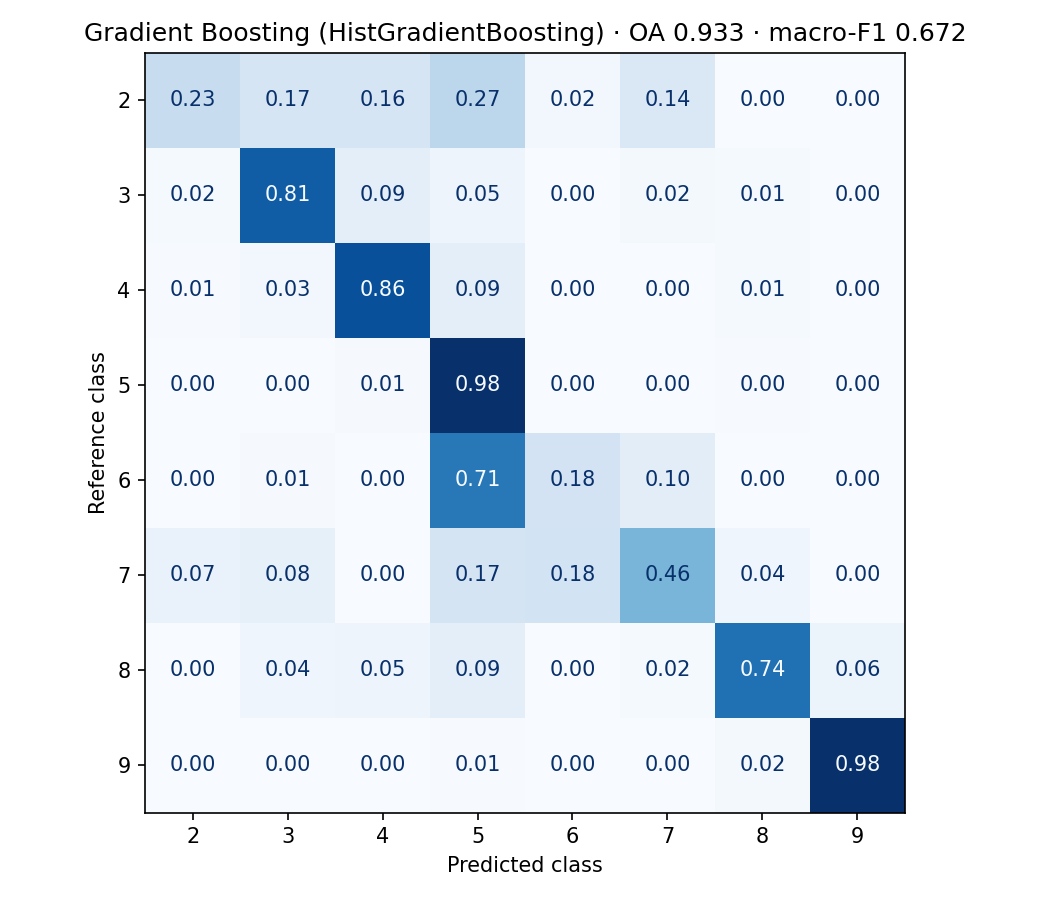
\includegraphics[width=\linewidth]{confusion_matrix_gradient_boosting}\end{subfigure}\hfill
\begin{subfigure}{0.24\linewidth}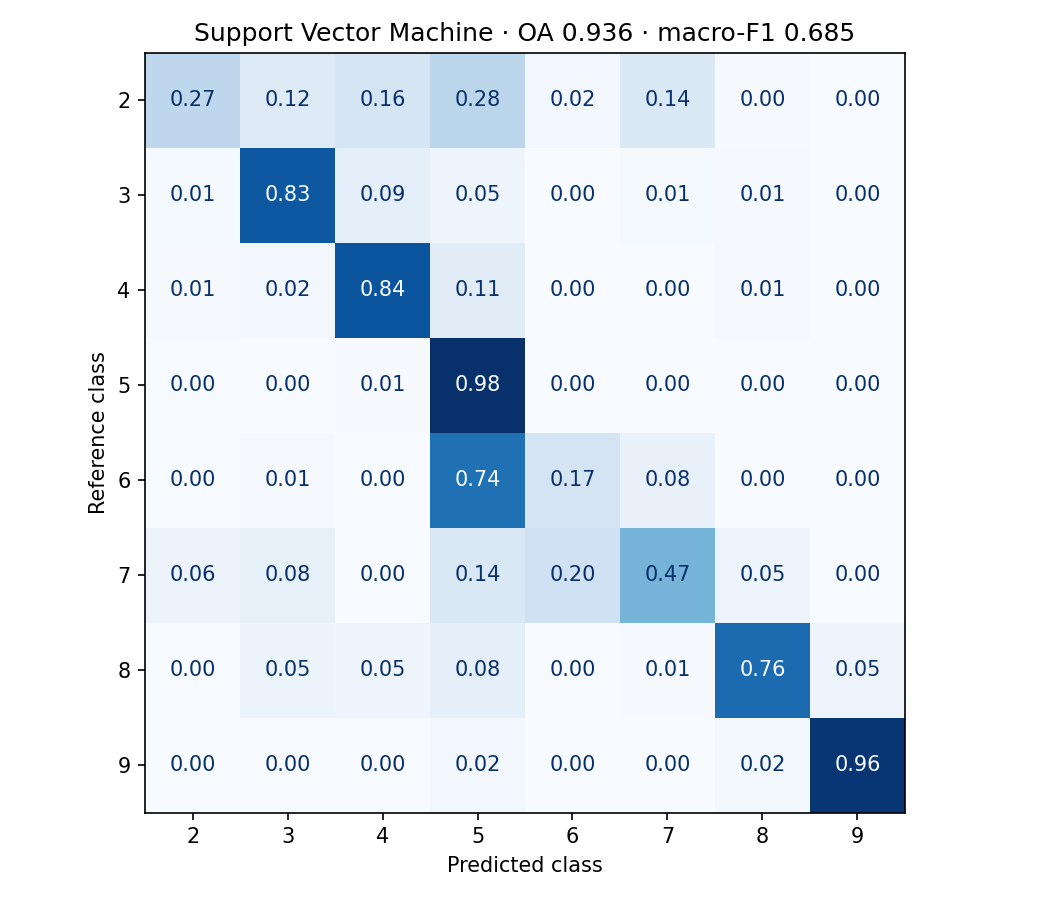
\includegraphics[width=\linewidth]{confusion_matrix_svm}\end{subfigure}\hfill
\begin{subfigure}{0.24\linewidth}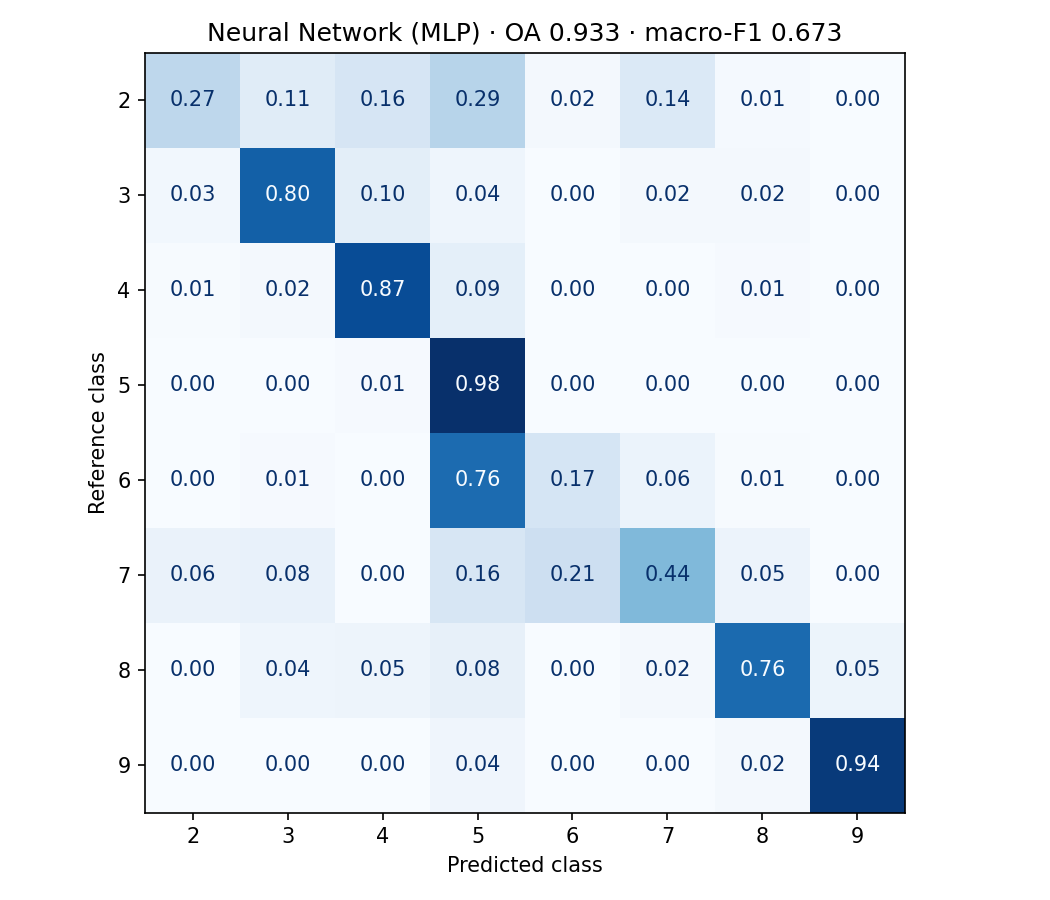
\includegraphics[width=\linewidth]{confusion_matrix_neural_network}\end{subfigure}
\caption{Normalised confusion matrices of the eight models on the test set.
First row: Logistic Regression, K-Nearest Neighbors, Naive Bayes, Decision
Tree. Second row: Random Forest, Gradient Boosting, Support Vector Machine,
neural network.}
\label{fig:allconfusion}
\end{figure}


\subsection{Most influential bands}

Decision trees show directly which bands drive the classification: every
question of the tree is a threshold on one band, and the importance of a band
is the share of the total class mixing removed by the questions on that band
(Figure~\ref{fig:bands}). The single tree relies above all on two bands at the
opposite ends of the spectrum: B01, the coastal aerosol band (27\,\%), which
is very bright over clouds and haze and dark over the ground, and B12, the
second short-wave infrared band (26\,\%), which separates bare and built-up
surfaces, bright in this band, from vegetation and water, which absorb it.
The near infrared (B8A) and the red (B04), the pair behind the vegetation
index, come next. The three red-edge bands (B05 to B07) are almost unused by
the tree, because they carry nearly the same information as B04 and B8A.

The forest spreads the importance much more evenly, because each of its trees
only sees a random half of the bands at each question; B01, B02, B04 and B11
lead, and the red-edge bands still contribute least. The importance of a band
is shared with the bands that resemble it, so a low value means that the band
adds little to the others, not that it carries no information.

\begin{figure}[H]
\centering
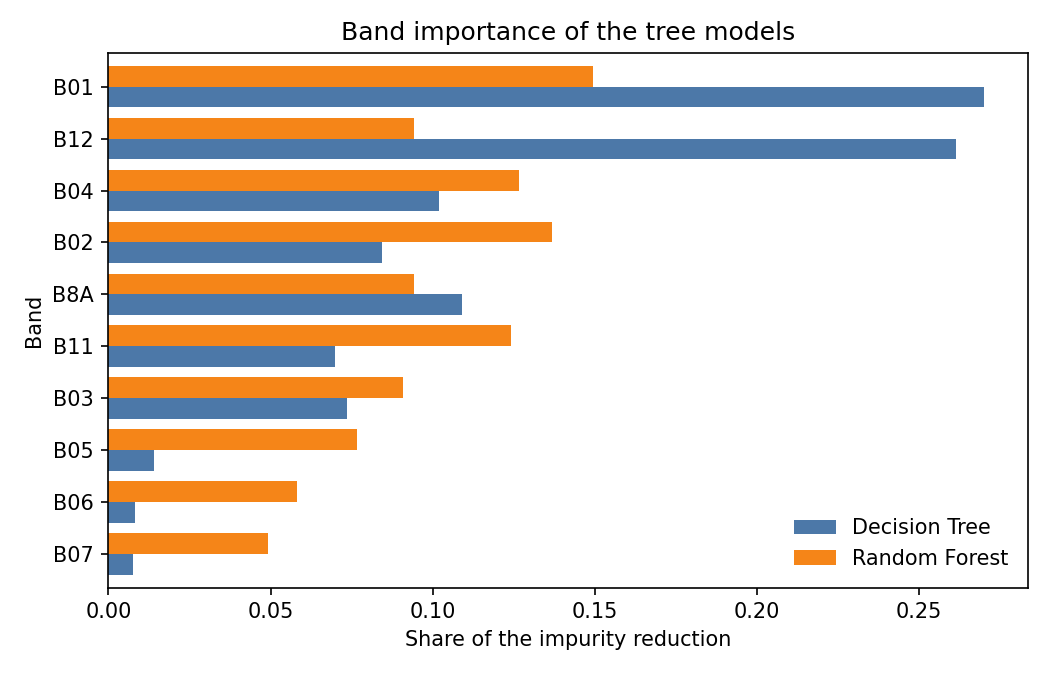
\includegraphics[width=0.6\linewidth]{band_importance}
\caption{Importance of each band in the Decision Tree and the Random Forest
(share of the total reduction of class mixing, Gini criterion; each model
sums to 1).}
\label{fig:bands}
\end{figure}

\section{Land-cover map of the scene}

\subsection{Final model and raster}

Once selected and evaluated, the Support Vector Machine was trained again with
the same configuration on all 583,835 labelled pixels, training and test
together, so that the map uses every reference polygon. The scores reported
above remain the estimate of its quality, because they were measured on
polygons the evaluated model had not seen. The final model keeps 70,887
support vectors (12\,\% of the labelled pixels), which shows how intricate the
boundaries between the dark classes are.

The model classified every pixel of the scene with data, 30,140,099 of the
30,140,100. The result is delivered as a single-band GeoTIFF,
\texttt{T18NWL\_20260810T152649\_landcover\_svm\_v1.tif}, with these
properties:

\begin{itemize}
  \item the grid of the source bands: $5490 \times 5490$ pixels of 20~m, the
  same origin and the coordinate reference system WGS~84 / UTM zone 18N
  (EPSG:32618), so it overlays the bands exactly in any GIS;
  \item one unsigned 8-bit value per pixel equal to the class label of the
  brief (2 to 10), and 255 for the pixel without data, a value that cannot be
  confused with a class (0 is a class of the convention);
  \item an embedded colour table with the colours of the brief, so it opens
  already styled.
\end{itemize}

The file was read again after writing to check its grid, its reference system
and its values, and it is stored in the project's object store. The model that
produced it is registered in the experiment tracker as the production version,
from which the project's prediction service loads it.

\subsection{Land-cover map}

Figure~\ref{fig:map} compares the true-colour image with the predicted map.
The main features of the scene are recognised: the urban area of Bogot\'a in
the south-east and the dry, bare hills of the west as non-vegetated surfaces,
the clouds over the centre and the south as cloud classes, the river that
crosses the scene from north to south as water, and the agricultural and
forested land that dominates the rest as vegetation.

\begin{figure}[H]
\centering
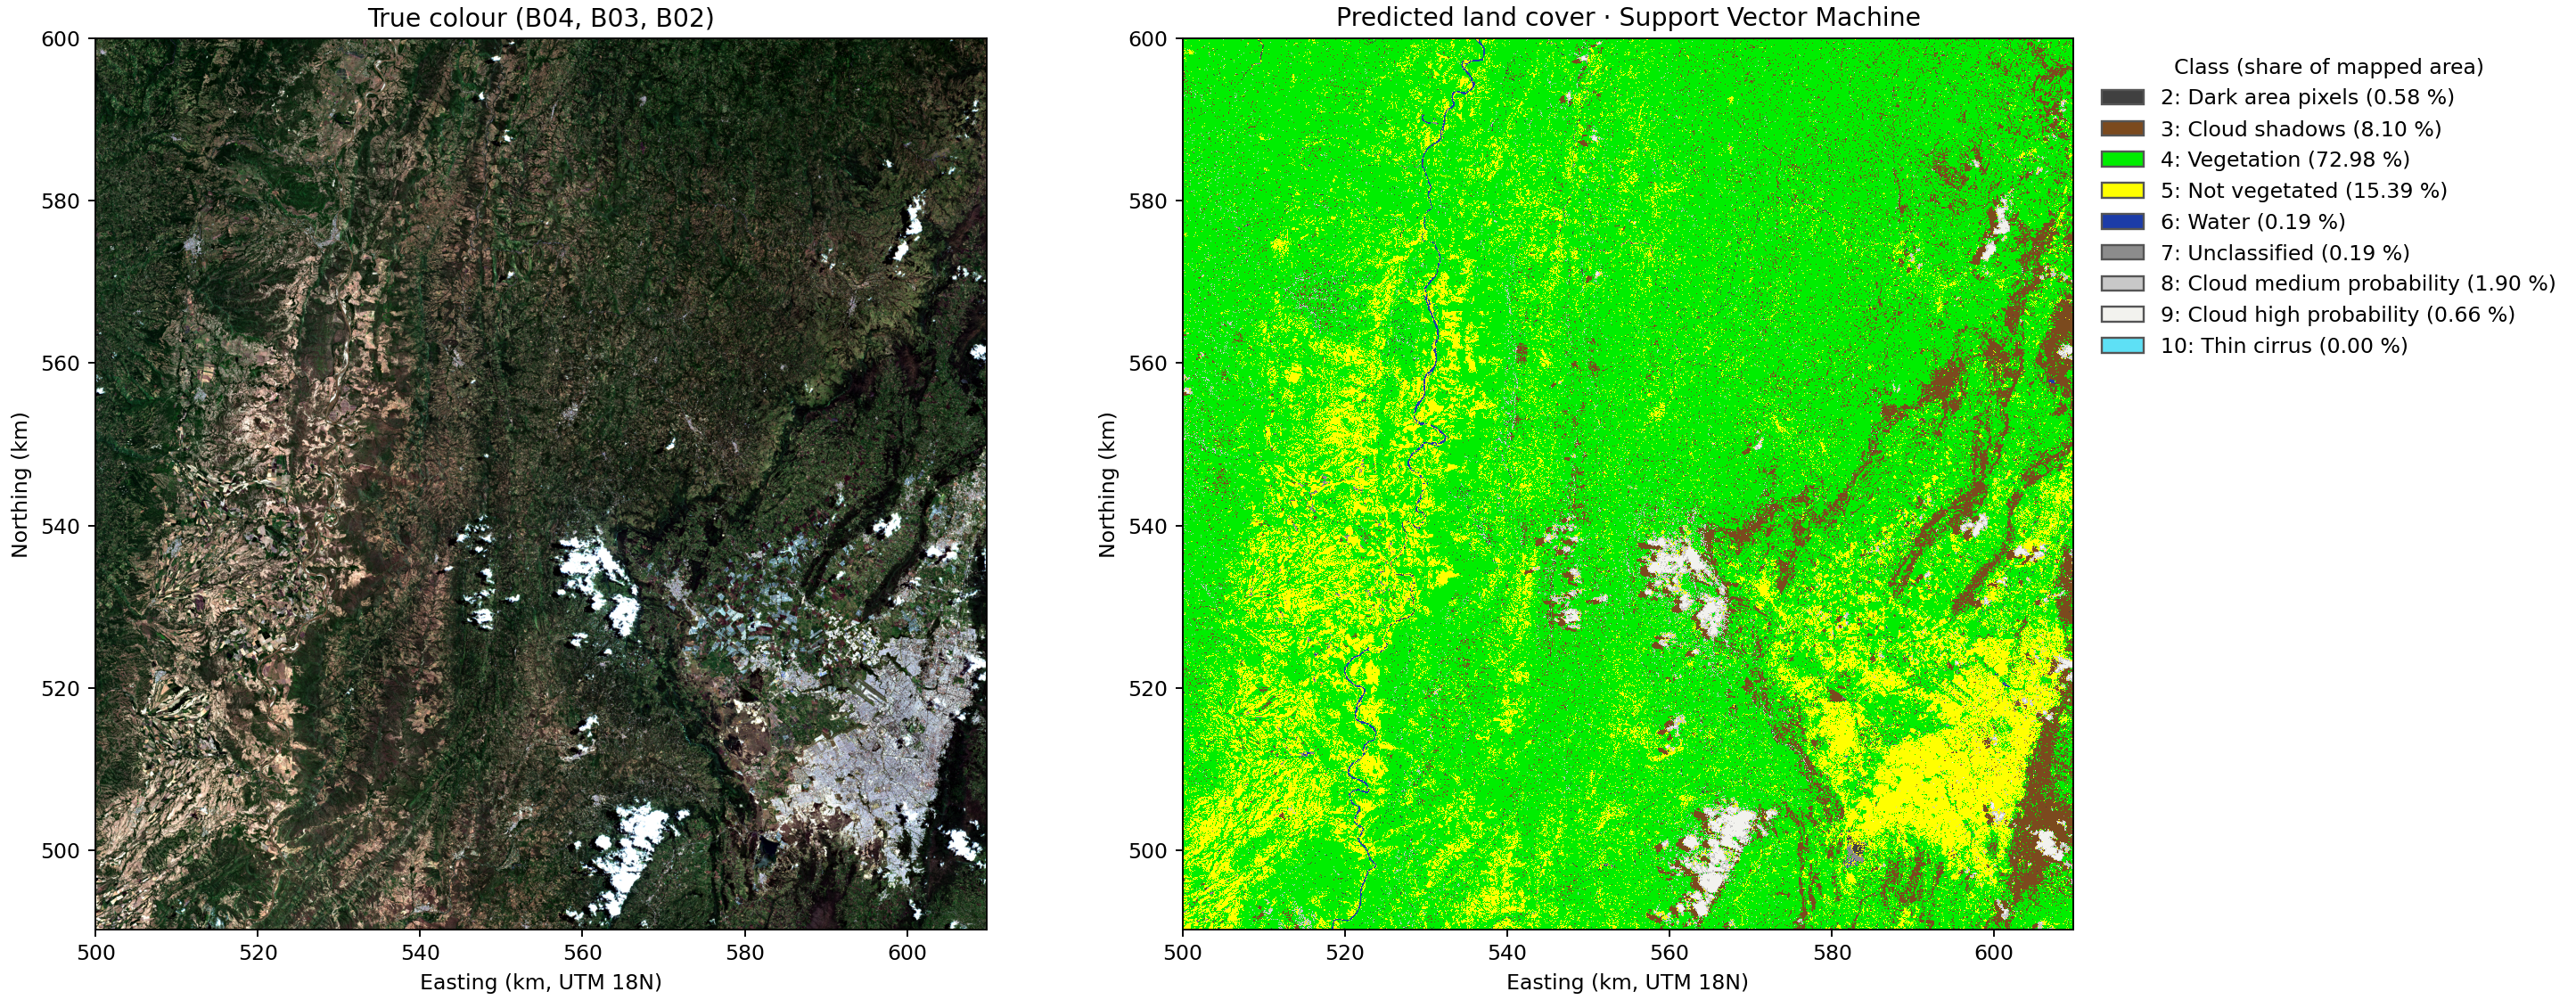
\includegraphics[width=\linewidth]{land_cover_map}
\caption{True-colour composite of the scene (left) and land cover predicted by
the Support Vector Machine (right). Coordinates in kilometres, UTM zone 18N.
The legend gives the share of the mapped area of each class.}
\label{fig:map}
\end{figure}

\subsection{Area per class}

The area of each class is the number of its pixels times the area of a pixel,
400~m$^2$ (0.04~ha), which is exact because the grid is in metres
(Table~\ref{tab:areas}). The classes add up to the 12,056.04~km$^2$ of the
scene with data.

\begin{table}[H]
\centering\small
\caption{Area of each predicted class over the whole scene.}
\label{tab:areas}
\begin{tabular}{clrrrr}
\toprule
Class & Land cover & Pixels & Area (ha) & Area (km$^2$) & Share (\%) \\
\midrule
2 & Dark area pixels & 175,078 & 7,003.12 & 70.03 & 0.58 \\
3 & Cloud shadows & 2,442,300 & 97,692.00 & 976.92 & 8.10 \\
4 & Vegetation & 21,996,588 & 879,863.52 & 8,798.64 & 72.98 \\
5 & Not vegetated & 4,639,459 & 185,578.36 & 1,855.78 & 15.39 \\
6 & Water & 58,687 & 2,347.48 & 23.47 & 0.19 \\
7 & Unclassified & 55,823 & 2,232.92 & 22.33 & 0.19 \\
8 & Cloud medium probability & 573,295 & 22,931.80 & 229.32 & 1.90 \\
9 & Cloud high probability & 198,426 & 7,937.04 & 79.37 & 0.66 \\
10 & Thin cirrus & 443 & 17.72 & 0.18 & 0.00 \\
\midrule
 & Mapped area & 30,140,099 & 1,205,603.96 & 12,056.04 & 100.00 \\
 & No data (code 255) & 1 & 0.04 & 0.00 & -- \\
\bottomrule
\end{tabular}

\end{table}

Vegetation covers 73.0\,\% of the scene and non-vegetated surfaces 15.4\,\%.
These shares are almost the reverse of the training dataset, where 73.6\,\% of
the pixels are not vegetated: the reference polygons concentrate on the city
and do not sample the scene at random. Cloud shadows cover 977~km$^2$, three
times the area of the clouds that should cast them (309~km$^2$). The map shows
why: steep forested slopes in the east of the scene, dark because they face
away from the sun, are classified as cloud shadow. Their spectra are very
close to those of a shadow, and the model sees each pixel alone, without its
neighbours or the terrain.

\section{Limitations}

\begin{itemize}
  \item \textbf{Reference sample.} The polygons were not drawn at random over
  the scene, and their class proportions differ widely from those of the map.
  The test scores describe how well the models reproduce the reference
  polygons; they are not an estimate of the accuracy of the map. Measuring it
  would require reference points drawn at random over the scene. The
  overall accuracy, dominated by class 5, says the least about the map, which
  is why the models were chosen by macro F1.
  \item \textbf{Rare classes.} Class 10 (thin cirrus) comes from a single
  polygon and cannot be evaluated, although the model can predict it. Water
  (17 polygons) and cloud shadows (58) are represented by few polygons, so
  their scores depend on a handful of them and vary strongly between
  validations.
  \item \textbf{Pixel by pixel, one date.} The models see only the ten values
  of each pixel on one date. Classes that are dark in every band (dark area
  pixels, water, shadows and shaded slopes) cannot be fully separated this
  way; the terrain (slope and orientation), the neighbouring pixels or a second
  date would help to tell a cloud shadow from a slope in shade.
  \item \textbf{Digital numbers.} Without the product metadata the models work
  on digital numbers instead of reflectance. This is harmless within the scene,
  but the model should not be applied to scenes processed with a different
  offset.
  \item \textbf{Extent of the search.} The best value of \texttt{C} of the
  Support Vector Machine and the largest architecture of the neural network
  are the largest values of their grids, so wider grids might improve them
  slightly. The five most costly models were compared on a quarter of the
  training pixels, which may favour slightly simpler configurations.
  \item \textbf{Cost of the selected model.} A Support Vector Machine compares
  every new pixel with all its support vectors, so classifying a full scene is
  much slower than with tree ensembles or the neural network, whose test
  scores are within 0.013 of macro F1.
\end{itemize}

\section{Conclusions}

\begin{enumerate}
  \item The complete chain, from the band files and the reference polygons to
  a georeferenced land-cover raster and its areas, runs in Python and is
  reproducible from the stored data, the notebooks and the tracked models.
  \item Splitting by polygon, both for the test set and for the validations,
  is essential: it makes every score an estimate on polygons the model has
  never seen, and it keeps all models comparable on the same data.
  \item With the macro F1 as criterion, the Support Vector Machine with a
  radial kernel on the logarithm of the bands is the best model, both on the
  ten validations (0.731) and on the test set (OA 0.936, kappa 0.849, macro F1
  0.685). The neural network and Gradient Boosting are close behind and are
  sensible alternatives when the cost of classifying many scenes matters.
  \item Models with flexible boundaries (kernels, networks, tree ensembles)
  clearly beat Logistic Regression and Naive Bayes, and the preparation of
  the features matters: the logarithm of the bands was chosen by every model
  that could use it, and trees need a minimum leaf size.
  \item Bright and well-represented classes are mapped reliably. Dark classes
  (dark area pixels, water, cloud shadows) remain the main source of error,
  both on the test set and on the map, where shaded slopes appear as cloud
  shadow. More reference polygons of these classes, terrain information and
  features from neighbouring pixels are the most promising improvements.
\end{enumerate}

\end{document}
